In this chapter we provide a real-world use-case that serves as motivation
for the rest of the work described in this dissertation. After giving
an introduction to the problem and related work in Section \ref{sec:session-length-background},
we describe the methods we used to analyze the data and make predictions in
Section \ref{sec:session-length-method} and summarize our findings in Section
\ref{sec:session-length-main-findings}. Finally, in Section \ref{sec:session-length-discussion} we provide desiderata
for a real-world system and identify gaps in the current state-of-the-art
research. We provide solutions to each of the
specific problems identified here in the following chapters.

\section{Background}
\label{sec:session-length-background}

As media streaming services have proliferated it has become important for streaming
companies to analyze their users' behavior to optimize their offering and
meet their business goals. One important factor in user satisfaction is the length of
users' sessions~\cite{dwell-time-satisfaction}, which we define as the
the complete interaction of a
user starting up the service, consuming a number of items, and ending
their interaction after some elapsed time.
This kind of interaction has been studied in the web search \cite{dwell-time-satisfaction, search-time-model} and ad click \cite{post-click-ads, post-click-survival}
domains, but no study had investigated the media streaming domain before.

Streaming services can use the length of user session to optimize their
recommendations, for example providing exploratory and more ``risky'' recommendations
for long sessions, versus exploitation and more ``safe'' recommendations for short sessions.
In ad-supported services, having an indication of the session length can also help
with scheduling ads, allowing the provider to meet their revenue target, while
minimizing the annoyance to the user~\cite{annoying-ads}.

Predicting the length of user sessions in a mobile streaming service can be challenging,
because user interaction lengths
typically exhibit long-tail distributions \cite{post-click-survival, weibull-web-browsing, phonecalls}, and the external factors that can influence the length of the
session can be hard to model, like users commuting, taking phone calls, or connectivity
issues. Media streaming sessions also differ from dwell time after ad clicks
and web search. In music specifically, which is the domain we are examining,
users typically consume multiple items in one session and have different behaviors
depending on the type of session as we show in our results (Section \ref{sec:session-length-main-findings}).

In our paper we provide an analysis the session length distribution using
tools from survival analysis and use build a predictive model using gradient boosted trees with specialized
loss functions to place the probability mass correctly in the presence of a
skewed dependent distribution.

\section{Analysis and Prediction of Media Streaming Session Length}
\label{sec:session-length-method}

In this section we describe the methods we have used to analyze the data
and create a predictive model for session length.

\subsection{Weibull Analysis of Session Length}

To analyze the user length behavior of the users we use tools from survival analysis~\cite{survival-analysis}, and specifically the Weibull distribution
\cite{weibull-survival}. The Weibull distribution is a flexible parametric distribution,
commonly used in survival analysis because it allows to model different kinds of failure
rates, where the probability of a unit failing changes over time. Its probability
density function is:

\begin{equation}
\label{eq:weibull-pdf}
f(t) = \frac{k}{\lambda}\left( \frac{t}{\lambda}\right)^{k-1}e^{-(t/\lambda)^k}, t \geq 0
\end{equation}


\noindent
that provides two parameters: the shape $k$ and the scale $\lambda$. The shape $k$ determines
the evolution of the failure rate over time, while the scale, $\lambda$, determines the spread
of the distribution. The effect of $k$ is best shown through an illustration of the hazard rate
for the Weibull function, that gives us the failure rate for an item that has survived until time
$t$, shown in Figure \ref{fig:weibull-failure-rate}.

\begin{figure}
	\centering
	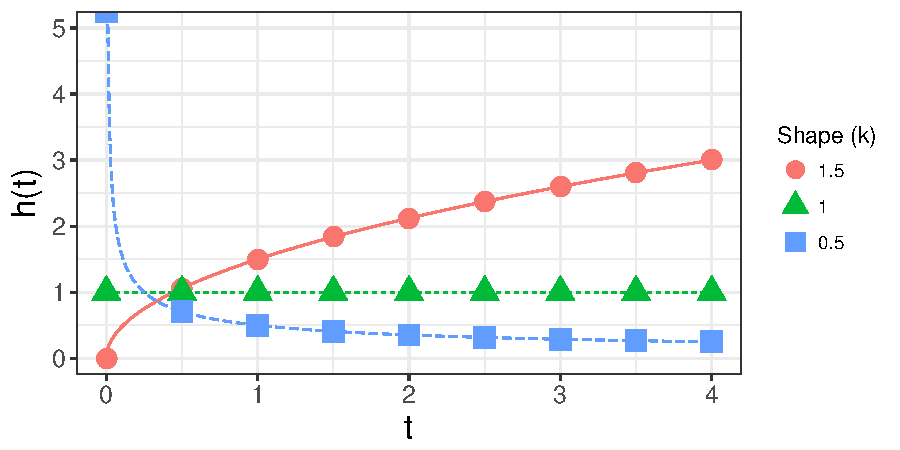
\includegraphics[width=0.7\textwidth]{weibull-hazard}
	\caption{The failure rate of the Weibull distribution for different values of the shape parameter, $k$. We set $\lambda = 1$.}
	\label{fig:weibull-failure-rate}
\end{figure}

The failure rate increases with time for $k > 1.0$, which is called the ``positive-aging''
effect, and decreases with time for $k < 1.0$ an effect called ``negative-aging''. Positive aging
is what we commonly associate with web sessions and is indeed observed in 98.5\% of post-click
behavior\cite{weibull-web-browsing}: as time goes on users become more likely to quit the session
at any point. On the other hand, negative aging means that sessions become less likely to end
as time goes on. This behavior is also described as ``infant mortality'' where defective units
may fail early on, but as time goes on they become less likely to fail.
For $k = 1$ the failure rate is constant and the distribution becomes equivalent to the
exponential distribution.

\subsection{Prediction}

On the prediction side, in order to tackle the issue of the long-tail distribution
of the sessions and to extract as much power as possible from the predictive features,
we choose the gradient boosted tree (GBT) algorithm. GBTs allow us to customize the
loss function to better fit the long-tail distribution of the dependent, and are flexible
enough to discover patterns in the large data we have available, and can readily
handle missing data which are common in industrial settings and our dataset in
particular.

We extracted a set of features for each user, like their gender, age, subscription
status (paid or free user), and a set of contextual features each session,
like the device type the session is on, the type of network (mobile, WiFi), or
the duration of the last session.

Our dependent is non-negative and long-tail distributed. One common solution in
these cases is to log-transform the dependent and then fit using a squared
loss, but we often want to use a loss function that is better suited to the
objective. To that end we try fitting the GBT both on the log-transformed data with
a mean squared error objective, as well as fitting on a log-likelihood
objective of a Gamma function with a log link function, which can explicitly
model non-negative data with a positive skew. We also test two versions
of each model: One where all data are aggregated and we build a single model,
and one where we build a personalized model for each user.


\section{Main Findings}
\label{sec:session-length-main-findings}

\subsection{User session distribution characteristics}

We use a dataset of user interaction from the Pandora music streaming service, which
is a major US-based music streaming service, and mainly ad supported. We define
sessions as periods of listening activity that are demarcated by breaks or pauses of
30 minutes or more.
We gather data from a random subset of users for the months of February to April 2016,
resulting in 4,030,755 sessions. We plot the normalized duration data in Figure
\ref{fig:session-length-times}.


\begin{figure}
	\centering
	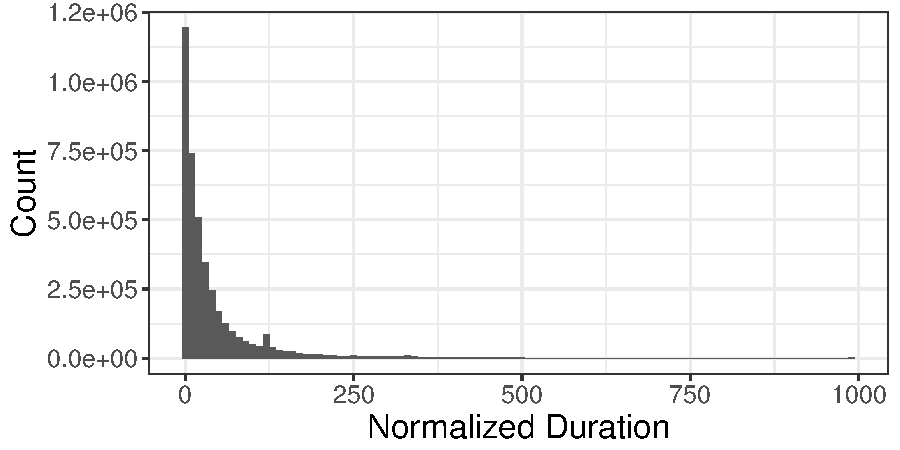
\includegraphics[width=0.7\textwidth]{duration-hist}
	\caption{Histogram plot of session length. The x-axis has been normalized to the 1-1000 range.}
	\label{fig:session-length-times}
\end{figure}

We analyze the session length distribution by fitting a Weibull distribution
to each user's data, and plot the resulting Empirical Cumulative Distribution
Function for the shape parameter in Figure \ref{fig:session-length-shapes}.
We can see that unlike the web site visits after a search, that had a negative aging
effect ($k < 1$) for 98.5\% of the users, only 44\% of the users exhibit
this behavior for music streaming. The behavior of the users is then split
roughly down the middle, with some users having sessions that become more likely
to end as time goes on, and others whose sessions become less likely to end as
they grow longer.


\begin{figure}
	\centering
	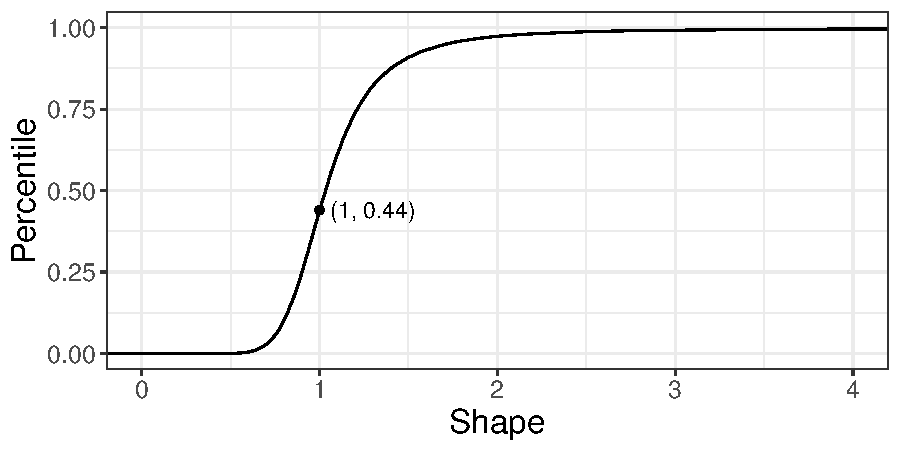
\includegraphics[width=0.7\textwidth]{weibull_shape_ecdf}
	\caption{The empirical cumulative distribution for the shape parameter per user.
		The x axis has been truncated at $x=4$ for readability (~99.5 \% of data points shown).}
	\label{fig:session-length-shapes}
\end{figure}

\subsection{Predictive model performance}

In our analysis of the performance of the predictive model we use two metrics.
We use the normalized Root Mean Squared Error which is a common choice
for regression problems, but also employ the normalized mean absolute error, a metric that is robust to outliers, to account
for the long-tail distribution of the dependent. For a baseline predictor we use the mean
session length per user, a heuristic that is simple, but personalized.
We present the results in Table
\ref{tab:session-length-prediction}.


\begin{table}
	\centering
	\caption{Performance metrics for length prediction task. We report the
		mean value across the 10 CV folds, and the standard deviation in parentheses.}
	\label{tab:session-length-prediction}
	\begin{tabular}{lll}
		\toprule
		Method (\textit{Objective}) & Normalized MAE & nRMSE \\
		\midrule
		Baseline & 1 \textit{(0.001)} & 1.16 \textit{(0.005)} \\
		Aggregated (\textit{MSE}) & \textbf{0.71} \textit{(0.008)} & 1.23 \textit{(0.008)} \\
		Aggregated (\textit{Gamma}) & 0.93 \textit{(0.007)} & \textbf{1.10} \textit{(0.005)} \\
		Per-user (\textit{MSE}) & 0.83 \textit{(0.002)} & 1.29 \textit{(0.004)} \\
		Per-user (\textit{Gamma}) & 0.86 \textit{(0.001)} & 1.31 \textit{(0.003)} \\
		\bottomrule
	\end{tabular}
\end{table}

From the results we can see that the aggregated models perform better overall,
something that can be explained by the fact that the per-user models are trained
on a few data points for most users, leading to over-fitting. The models using the
MSE objective place most of their probability mass closer to the origin and as a
result perform better in terms of MAE, but miss many of the longer sessions
and as a result perform worse in terms of RMSE.

\section{Discussion}
\label{sec:session-length-discussion}

In this chapter we presented our work on the analysis of session
length distribution in media streaming, and presented a specialized
predictive model.
Through this work we are able to identify several limitations in the current
state of the art in decision tree learning.

First, this work demonstrated the need for algorithms that are
able to learn online and adapt to a constantly changing environment. When
providing estimates of users' session length, we want the predictions of
the algorithms to adapt to the patterns exhibited throughout the day,
such as day/night and work/home cycles, and be able to adjust to drifting
distributions.
In order to be able to continuously adapt our models, we have focused on online learning
methods in Papers \boostvhtNum and \uncertaintreesNum that are both scalable and can continuously update tree models with new information about the world.

Second, we were able to identify the importance of quantifying the uncertainty
in predictions. For a quantity such as session length, exact predictions can
be of little value.
The ability to quantify the uncertainty in a prediction can be more useful as
it allows us to make decisions with confidence and avoid giving users
a bad experience.
For example, if we know with a high degree of certainty
that the true value of the session length will be between 30 and 45 minutes
we can optimize recommendations and ad scheduling for a long running session.
While there exist methods that are able to provide uncertainty estimates
from decision trees for static datasets, no methods exist for online decision trees.
\uncertaintrees
fills this gap in research that provides online decision trees models
with the ability to provide uncertainty estimates.

Finally, during this study we were able to get first hand experience with
the accuracy, flexibility and scalability that boosted decision trees
provide. The success of boosted trees has been well-documented,
from winning data mining competitions \cite{xgboost}, to being the model of choice for mission-critical
applications such as ad targeting at major enterprises \cite{mcrank, ctr-facebook}.
What's common in these applications is the need to deal with potentially very
high-dimensional data at scale.
In our follow-up work, we have focused on expanding the
area of scalable boosted trees for high-dimensional data in Paper \boostvhtNum in the online
domain, and Paper \blockgbtNum in the batch domain.